\documentclass[11pt]{article}
\usepackage[margin=1in]{geometry}
\usepackage{graphicx}
\usepackage{amsmath}
\usepackage{booktabs}
\usepackage{siunitx}
\usepackage{xcolor}
\usepackage{caption}
\usepackage[colorlinks=true,linkcolor=blue!55!black,urlcolor=blue!55!black]{hyperref}
\captionsetup{font=small,labelfont=bf}
\graphicspath{{figs/}}
\newcommand{\ns}{\,\mathrm{ns}}
\newcommand{\dmm}{\,\mathrm{mm}}
\newcommand{\vdr}{$v_\mathrm{drift}=34.30\,\mu\mathrm{m/ns}$}
\title{\vspace{-1.5em}Time resolution of the MX17 resistive Micromegas in micro-TPC mode\\
\large June 2026 cosmic bench --- det3 (\texttt{sat\_det3}) with det2 cross-check}
\author{MX17 cosmic-bench analysis (paper topic 10)}
\date{2026-07-11}

\begin{document}
\maketitle
\vspace{-1.5em}

\begin{abstract}
\noindent We measure the time resolution of the MX17 resistive-strip Micromegas
detectors operated in micro-TPC mode on the June cosmic bench. Contrary to an
earlier ``not feasible'' assessment, the bench \emph{does} carry an absolute time
reference: acquisition is triggered by a top+bottom scintillator-paddle
coincidence, and the DREAM readout applies the 3-bit fine timestamp
(\texttt{ftst}, \SI{10}{ns} granularity) that re-references the free-running
\SI{60}{ns} sampling clock to the trigger. We verify the fine-timestamp
correction directly in the data. Three complementary numbers follow, all on the
frozen data set: (i) a single-strip time resolution of
$\sigma_t=\SI{38.9}{ns}$ ($1.33\dmm$ of drift); (ii) a clean, telescope- and
geometry-free \emph{detector} resolution from the agreement of the two orthogonal
readout layers, $\sigma_t=\SI{33.1}{ns}$ per plane ($1.13\dmm$;
\SI{29.0}{ns}=$1.00\dmm$ after a residual time-walk correction), with an
inter-plane bias consistent with zero ($-1.3\ns$); and (iii) an absolute
event-time resolution (leading edge relative to the trigger) of
$\sigma_{68}=\SI{37.7}{ns}$, whose error budget is dominated by the detector term,
not by the trigger. det2 reproduces every number within ${\sim}10\%$. The
$\approx\SI{1}{mm}$-of-drift timing precision matches the transverse spatial
resolution --- the micro-TPC is not timing-limited relative to its geometry.
\end{abstract}

\section{The question, and what ``time resolution'' means here}
Hit mode answers \emph{where} a muon crossed; micro-TPC mode adds \emph{when} each
drift electron arrived, which is what turns a single plane into a 3-D track
segment. The relevant performance number is therefore the precision of the
per-strip arrival time and of the event timestamp it defines. Two distinct
questions hide under ``time resolution'':
\begin{itemize}
  \item \textbf{Absolute / time-of-flight:} how well does the detector timestamp
        the muon relative to an external clock? This needs a trigger reference.
  \item \textbf{Intrinsic / detector:} how reproducibly does the detector time an
        event using only its own channels? This is the number that limits
        micro-TPC tracking, independent of the trigger quality.
\end{itemize}
We measure both. The key enabler --- and the correction to the earlier
assessment --- is that the absolute reference is present.

\section{The timing chain: how an absolute time is formed}
\label{sec:chain}
The per-strip time is reconstructed in \texttt{mm\_strip\_reconstruction}
(\texttt{WaveformAnalyzer.cpp}) as a \textbf{constant-fraction} leading-edge
crossing: the waveform is walked down from its peak to $30\%$ of the
baseline-subtracted amplitude and linearly interpolated between the two bracketing
\SI{60}{ns} samples, giving a sub-sample time (Fig.~\ref{fig:algo}, right). Because
the threshold tracks each pulse's own amplitude, this is largely free of
amplitude time-walk by construction --- a point we confirm quantitatively in
Sec.~\ref{sec:single}.

The DREAM \SI{60}{ns} sampling clock is \emph{free-running} with respect to the
trigger. When the scintillator coincidence fires, the readout window opens at
whatever phase the clock happens to be in; that phase is recorded by the 3-bit
fine timestamp \texttt{ftst} ($0$--$7$, \SI{10}{ns} steps from the \SI{100}{MHz}
clock). The reconstruction \textbf{adds} $\texttt{ftst}\times\SI{10}{ns}$ to every
strip time (Fig.~\ref{fig:algo}, left), re-referencing the window start to the
trigger to \SI{10}{ns} granularity. The result is that each strip's \texttt{time}
is an absolute leading-edge time relative to the (phase-corrected) trigger.

\begin{figure}[h]
  \centering
  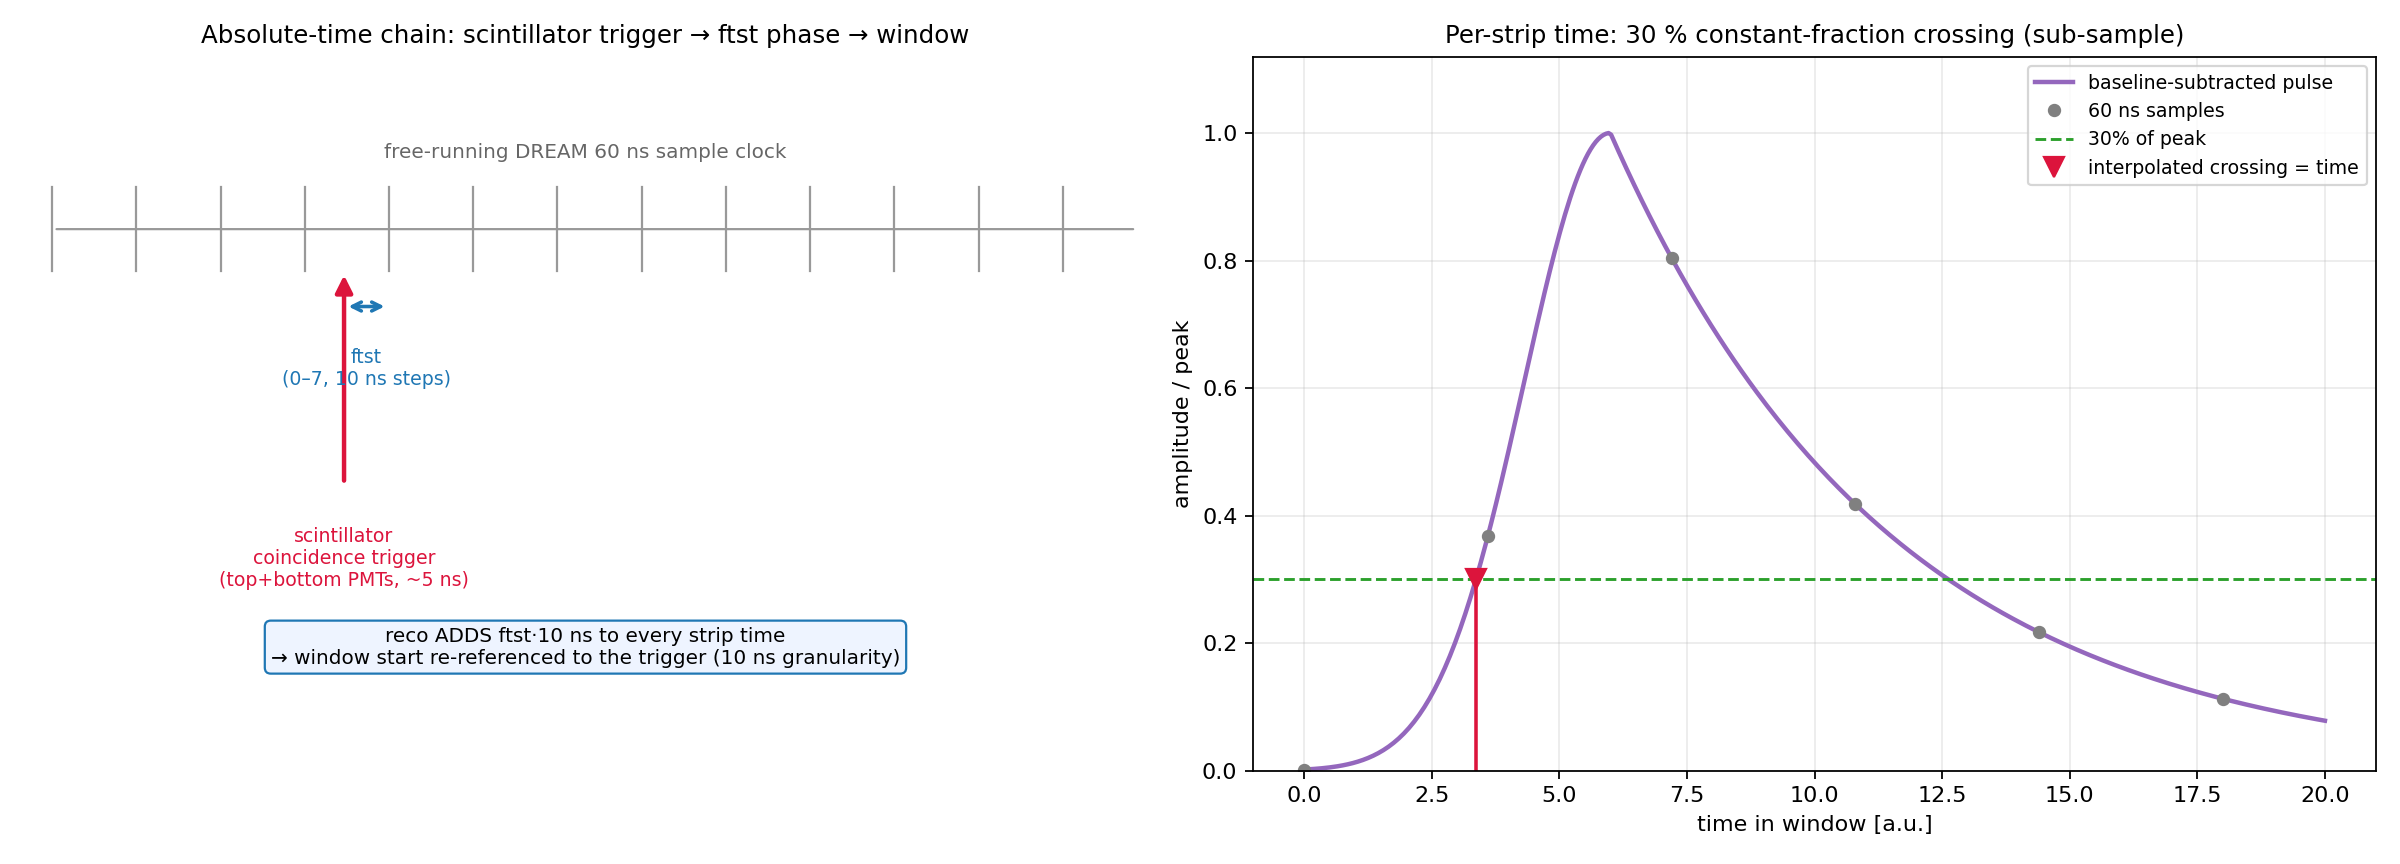
\includegraphics[width=\textwidth]{algorithm_schematic.png}
  \caption{The absolute-time chain. \emph{Left:} the scintillator-coincidence
  trigger arrives at a random phase of the free-running \SI{60}{ns} DREAM clock;
  \texttt{ftst} records that phase (\SI{10}{ns} steps) and the reconstruction adds
  it back to every strip time. \emph{Right:} the per-strip \texttt{time} is a
  $30\%$-of-peak constant-fraction crossing, linearly interpolated to sub-sample
  precision.}
  \label{fig:algo}
\end{figure}

\paragraph{The fine-timestamp correction, verified in data.}
If the \texttt{ftst} correction were \emph{not} applied, the reconstructed event
time would slide by \SI{10}{ns} per \texttt{ftst} unit. As applied, the leading-edge
event time is flat in \texttt{ftst} (slope $-0.2\ns$/step); undoing the correction
restores the expected $-10.2\ns$/step (Fig.~\ref{fig:ftst}, left). Correcting the
phase also tightens the absolute event-time distribution from
$\sigma_{68}=\SI{41.3}{ns}$ to \SI{37.7}{ns} (Fig.~\ref{fig:ftst}, right). This is
direct evidence that the sampling phase is measured and removed, i.e.\ that an
absolute time exists.

\begin{figure}[h]
  \centering
  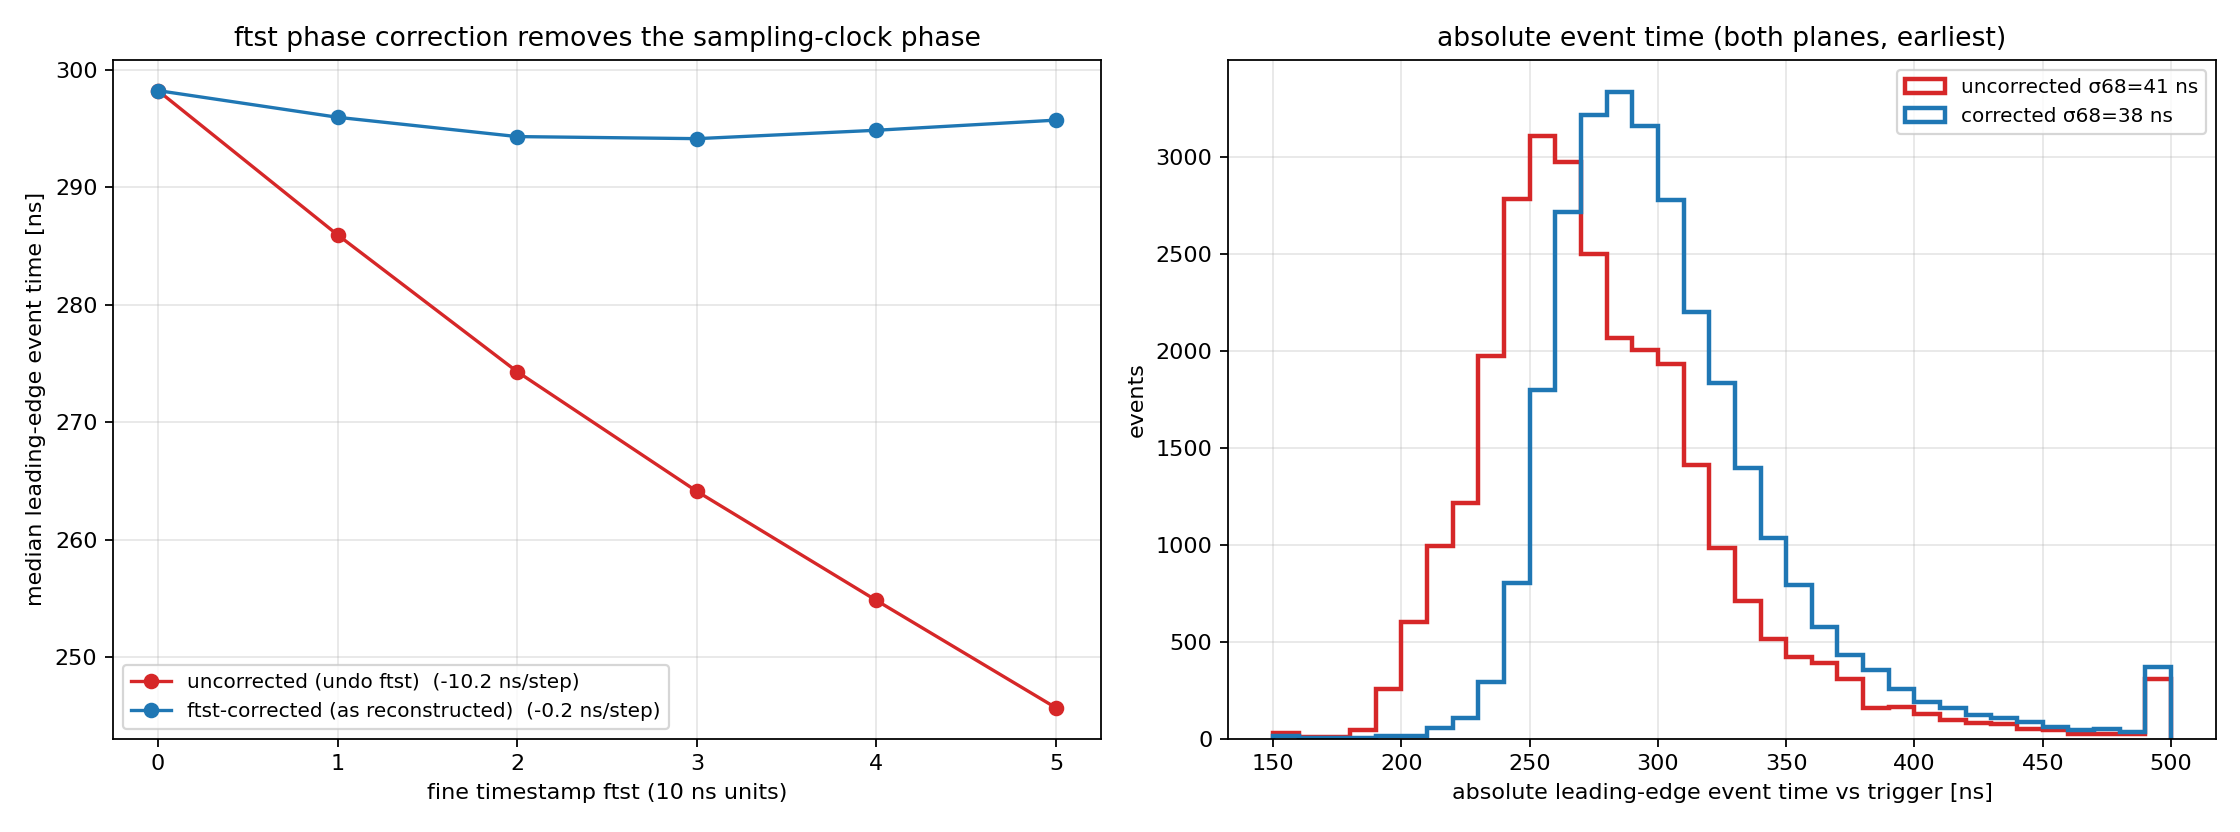
\includegraphics[width=\textwidth]{ftst_correction.png}
  \caption{Fine-timestamp phase correction. \emph{Left:} median leading-edge event
  time vs \texttt{ftst}; the applied correction (blue) is flat, the uncorrected
  case (red) walks by $-10\ns$/step. \emph{Right:} the absolute event-time
  distribution is tighter with the correction applied.}
  \label{fig:ftst}
\end{figure}

\section{Method: three observables}
All observables use the detector's own combined hits (spark/multiplicity veto
$\le 50$ strips, hit amplitude $>100$~ADC, pulse-start time in $(0,2000)\ns$). Per
event and plane we take the largest spatial strip cluster ($\ge 3$ strips).
Nothing here uses the M3 telescope --- the measurement is self-contained. We adopt
\vdr (the \texttt{sat\_det3} geometric drift
velocity at \SI{1000}{V}) to translate a time to an equivalent drift distance,
$\sigma_z = v_\mathrm{drift}\,\sigma_t$.

\begin{description}
  \item[A. Single-strip $\sigma_t$.] For inclined tracks the core strips
  (amplitude $\ge 30\%$ of the cluster max, $\ge 4$ strips spanning $\ge \SI{2}{mm}$)
  fall on a line $\mathrm{time}(\mathrm{position})$. The $(N{-}2)$-normalised RMS of
  the residual is the per-strip timing precision.
  \item[B. Plane-to-plane detector $\sigma_t$.] The X and Y strip layers sit under
  \emph{one} drift gap and collect the \emph{same} drifting electrons
  (Fig.~\ref{fig:geom}), so the shortest-drift charge produces the same
  leading-edge time in both layers. The two layers are two \emph{independent}
  measurements of one event timestamp: $\sigma(t_X{-}t_Y)/\sqrt2$ is the
  single-plane detector resolution, and the median of $t_X{-}t_Y$ is the residual
  inter-plane time-walk (a bias). Differencing cancels the trigger, the
  \texttt{ftst} phase, and the drift geometry, isolating the detector.
  \item[C. Absolute event-time $\sigma_{68}$.] The earliest leading-edge time of
  the event (either plane), relative to the phase-corrected trigger. This is the
  time-of-flight-style number; it is an upper limit because it still contains the
  event-to-event variation of the minimum drift distance.
\end{description}

\begin{figure}[h]
  \centering
  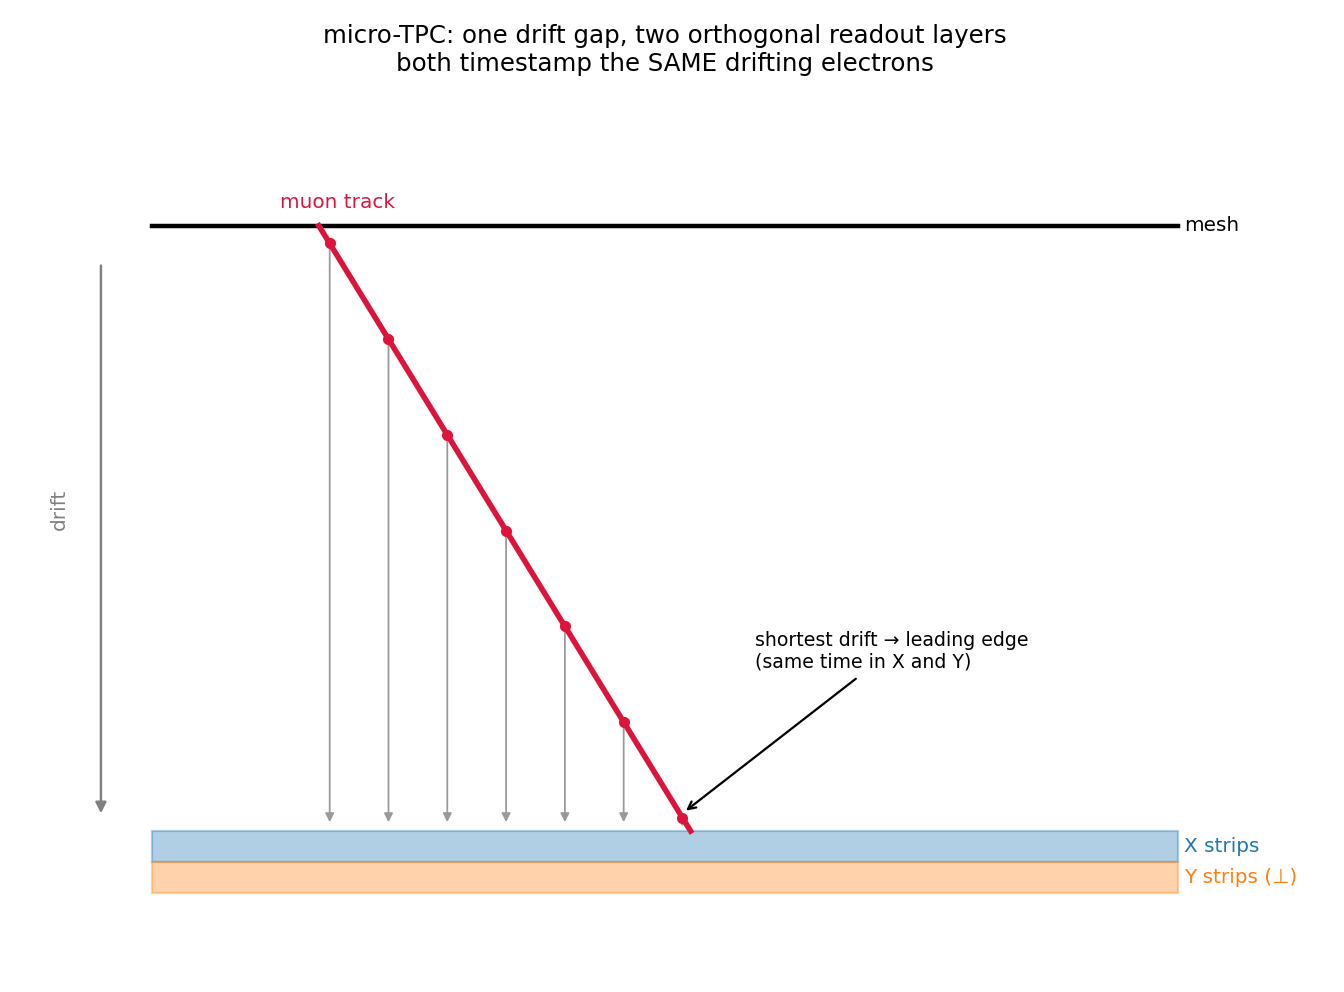
\includegraphics[width=0.62\textwidth]{geometry_schematic.png}
  \caption{Micro-TPC geometry. A single drift gap and mesh above two orthogonal
  strip layers; every drift electron induces on an X and a Y strip at the same
  time, so the two planes independently time the same arrival sequence. The
  shortest-drift ionization sets the event leading edge.}
  \label{fig:geom}
\end{figure}

\section{Results (det3, \texttt{sat\_det3}, \num{28404} dual-plane events)}

\subsection{A. Single-strip time resolution}
\label{sec:single}
The per-strip residual has a median $\sigma_t=\SI{38.9}{ns}$
($=1.33\dmm$ of drift; x/y $=39.2/38.6\ns$; Fig.~\ref{fig:single}, left). The
per-strip \emph{time-walk} --- the residual as a function of the strip's relative
amplitude --- is only $+3\ns$ per unit relative amplitude
(Fig.~\ref{fig:single}, right), i.e.\ negligible. This confirms that the
$30\%$ constant-fraction crossing already removes amplitude walk at the single-strip
level, so no per-strip walk calibration is needed for the track fit.

\begin{figure}[h]
  \centering
  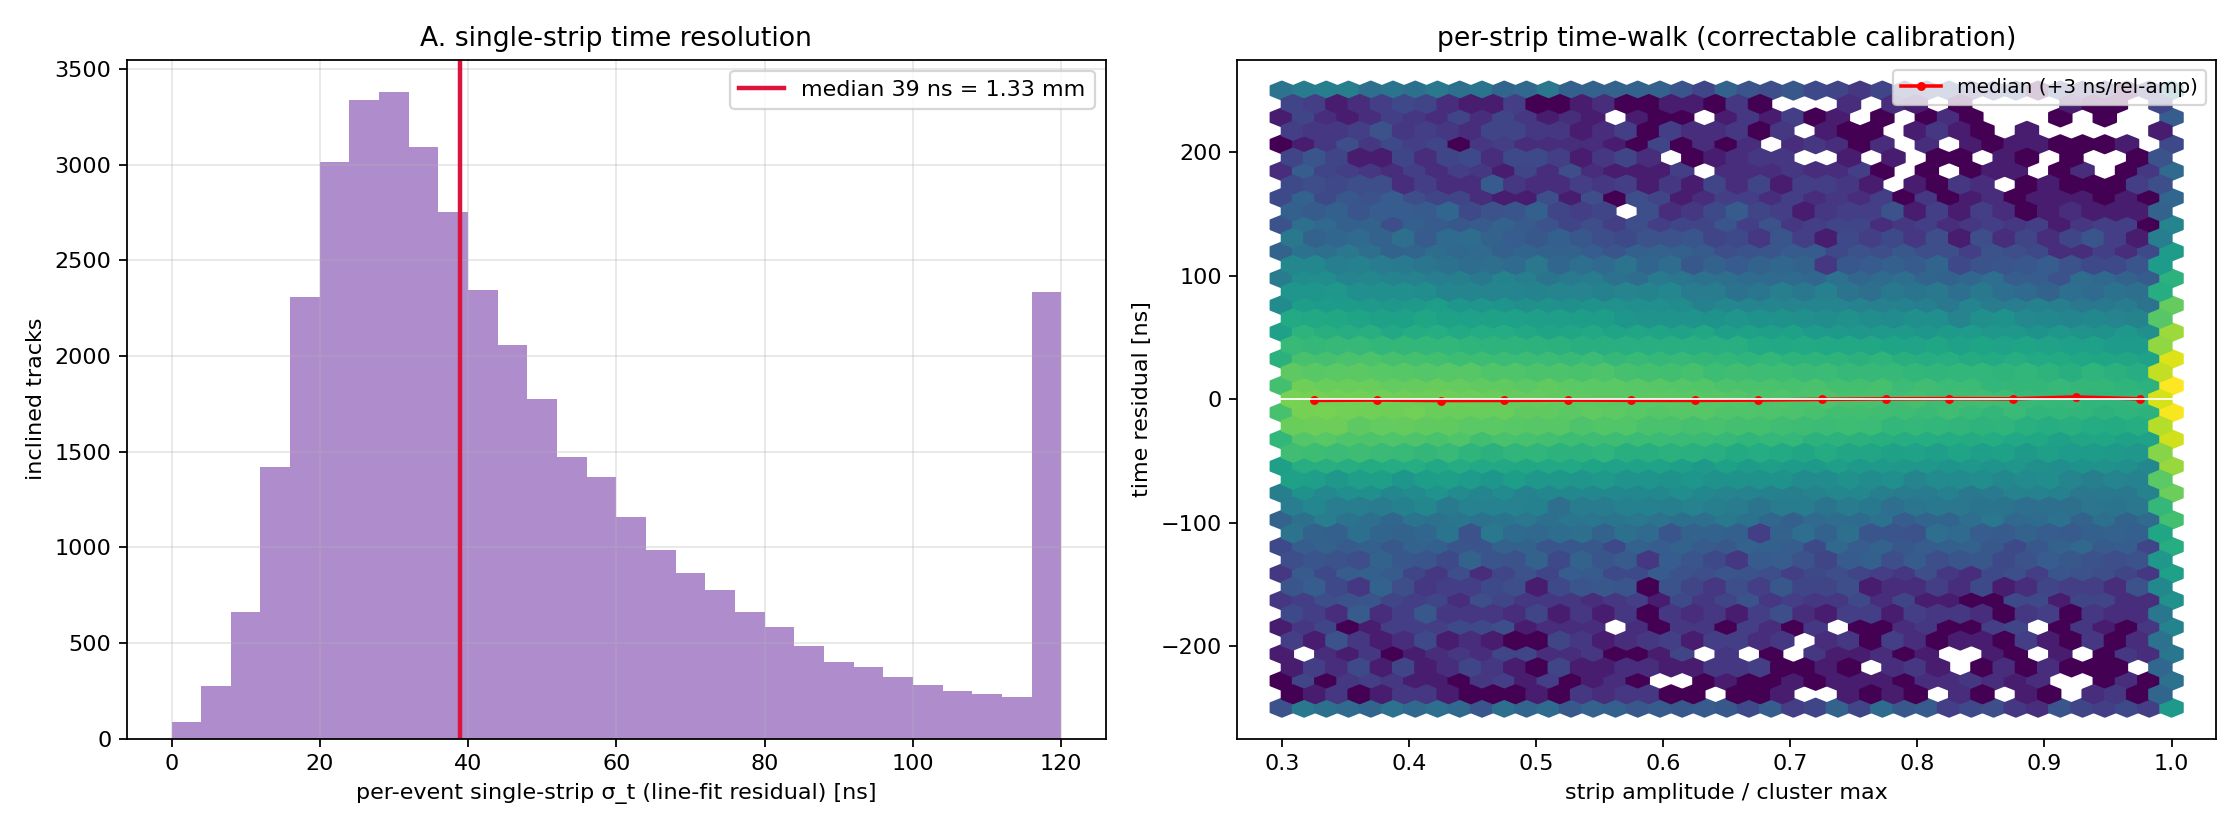
\includegraphics[width=\textwidth]{single_strip.png}
  \caption{\emph{Left:} single-strip time resolution from the micro-TPC line-fit
  residual. \emph{Right:} per-strip time residual vs relative amplitude --- the
  near-flat trend ($+3\ns$/rel-amp) shows the constant-fraction timing is
  walk-free at the strip level.}
  \label{fig:single}
\end{figure}

\subsection{B. Plane-to-plane detector resolution (headline)}
The two layers agree with an inter-plane bias of $-1.3\ns$ --- consistent with
zero --- directly confirming the ``one gap, two orthogonal readouts of the same
arrivals'' picture. The spread gives a single-plane detector resolution of
$\sigma_t=\SI{33.1}{ns}$ ($1.13\dmm$; Fig.~\ref{fig:ptp}, left). A residual
inter-plane time-walk correlated with the plane charge asymmetry
($-105\ns$ per unit asymmetry; Fig.~\ref{fig:ptp}, right) --- the brighter plane
crosses threshold slightly earlier --- is correctable, taking the resolution to a
floor of \SI{29.0}{ns} ($1.00\dmm$). The leading edge is by far the sharpest event
estimator: the median strip time gives \SI{70.3}{ns} per plane, and the trailing
(mesh-side) edge is worse still, as expected from longitudinal diffusion.

\begin{figure}[h]
  \centering
  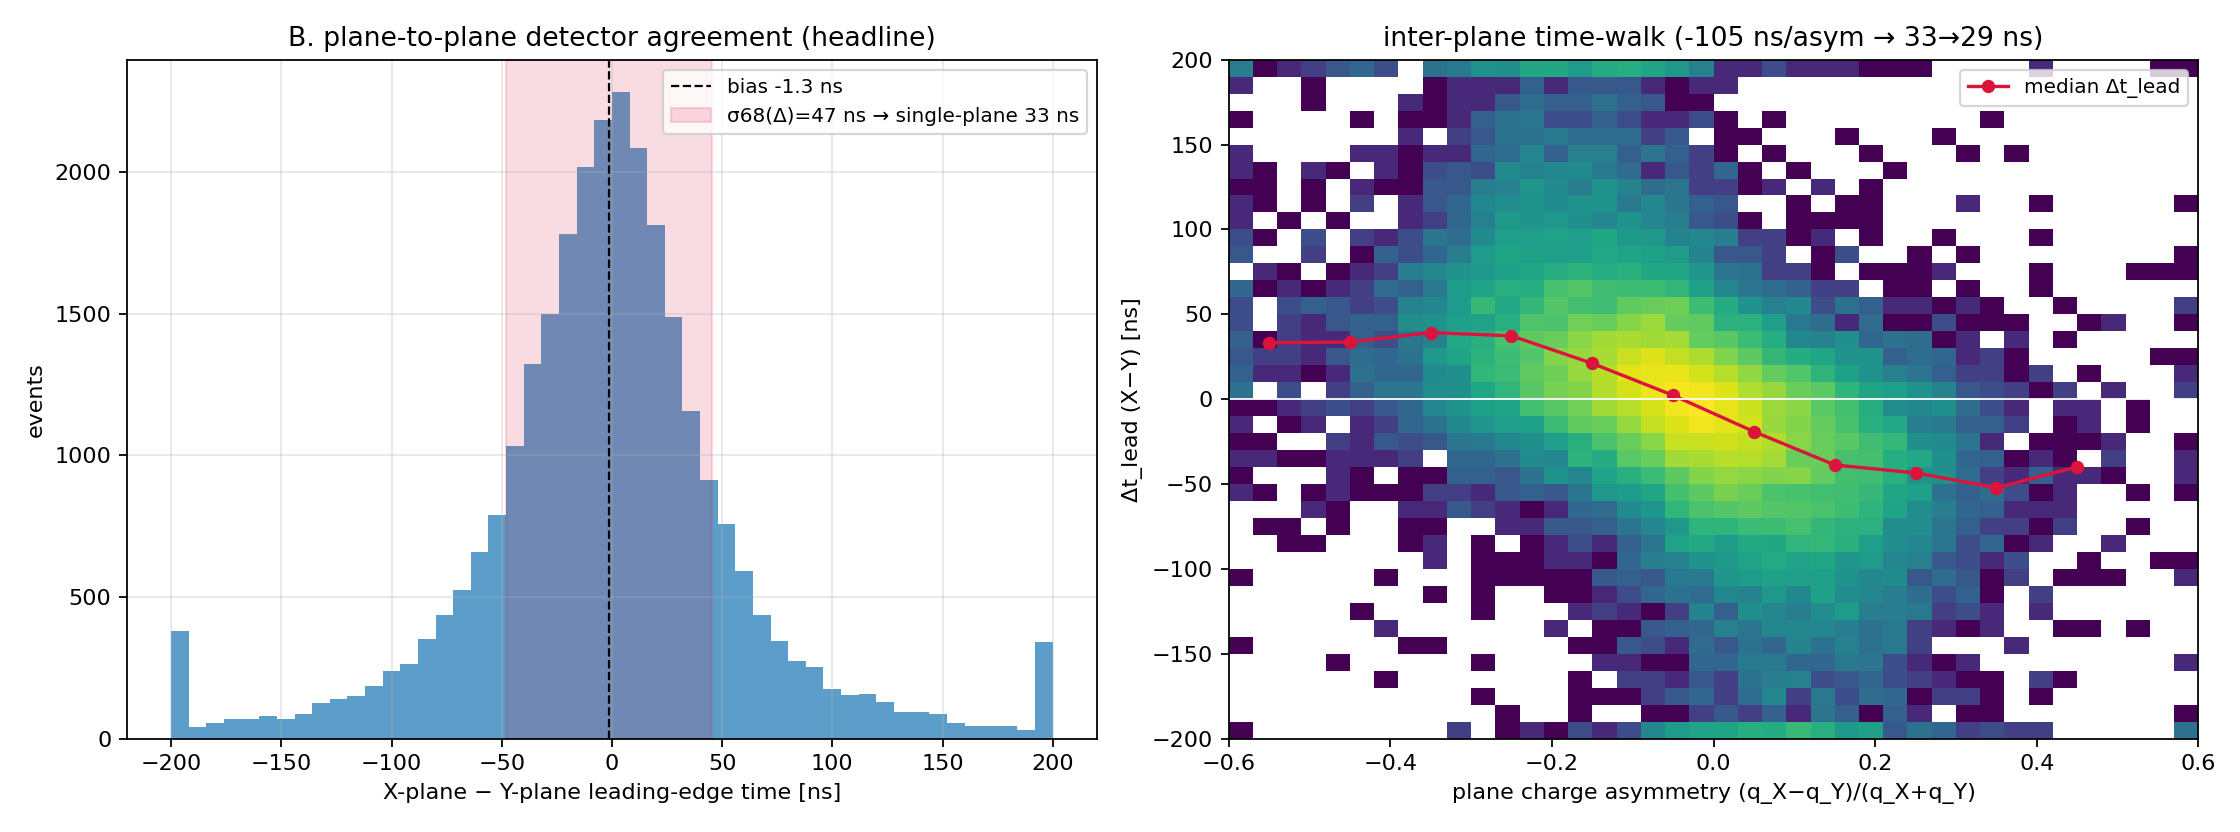
\includegraphics[width=\textwidth]{plane_to_plane.png}
  \caption{\emph{Left:} X$-$Y leading-edge time difference; bias $\approx 0$ and
  $\sigma_{68}(\Delta)=\SI{47}{ns}\Rightarrow$ single-plane \SI{33}{ns}.
  \emph{Right:} the residual inter-plane time-walk vs plane charge asymmetry; its
  removal takes the resolution from 33 to \SI{29}{ns}.}
  \label{fig:ptp}
\end{figure}

\subsection{C. Absolute event-time resolution and its budget}
The absolute leading-edge event time has $\sigma_{68}=\SI{37.7}{ns}$
(Fig.~\ref{fig:ftst}, right), an upper limit because it still folds the drift
geometry. Decomposing $\sigma_\mathrm{abs}^2 = \sigma_\mathrm{det}^2 +
\sigma_\mathrm{scint}^2 + \sigma_\mathrm{ftst}^2 + \sigma_\mathrm{geom}^2$ with the
detector term from (B), the scintillator pair ${\sim}\SI{5}{ns}$, and the
fine-timestamp quantization $\SI{10}{ns}/\sqrt{12}=\SI{2.9}{ns}$, leaves a
geometry term of ${\sim}\SI{17}{ns}$. \textbf{The absolute time budget is
dominated by the detector}, not by the trigger: the scintillator and the
\texttt{ftst} granularity are subdominant.

\subsection{Time resolution vs drift depth}
Binning the plane-to-plane resolution by the event's leading-edge drift time
(Fig.~\ref{fig:depth}) shows $\sigma_t$ rising from ${\sim}\SI{28}{ns}$
(${\sim}\SI{1}{mm}$) for tracks reaching close to the readout to $>\SI{150}{ns}$ for
tracks whose earliest charge is already deep in the gap. The growth is steeper than
pure diffusion, reflecting the additional signal-to-noise loss from electron
attachment (the same $\lambda\approx\SI{15}{mm}$ attachment that sets the drift-gap
story).

\begin{figure}[h]
  \centering
  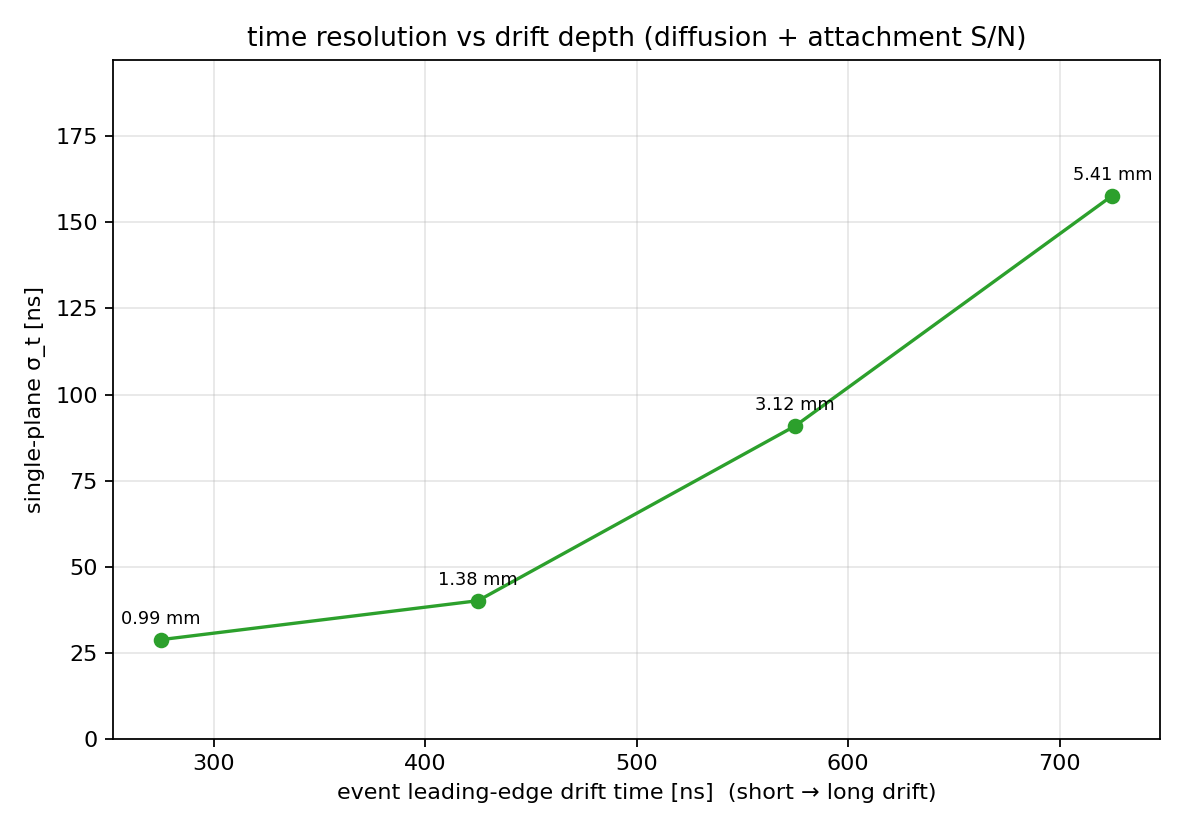
\includegraphics[width=0.6\textwidth]{drift_depth.png}
  \caption{Single-plane detector $\sigma_t$ vs event drift depth. Short drift
  (${\sim}\SI{1}{mm}$) is best; the rise with depth is diffusion plus
  attachment-driven S/N loss.}
  \label{fig:depth}
\end{figure}

\section{Cross-check: det2 replication}
Repeating the analysis on an independent detector (\texttt{o22\_long\_det2},
\SI{525}{V}, different FEU pair, \num{23894} dual-plane events) reproduces every
number within ${\sim}10\%$ (Table~\ref{tab:results}), establishing these as a
design/gas property rather than a per-chamber accident.

\begin{table}[h]
  \centering
  \caption{Time-resolution summary. Drift-distance equivalents use
  \vdr.}
  \label{tab:results}
  \begin{tabular}{lccc}
    \toprule
    Quantity & det3 (\texttt{sat\_det3}) & det2 (\texttt{o22\_long\_det2}) & equiv.\ drift \\
    \midrule
    Single-strip $\sigma_t$              & \SI{38.9}{ns} & \SI{40.5}{ns} & $1.33/1.39\dmm$ \\
    Detector $\sigma_t$ (leading edge)   & \SI{33.1}{ns} & \SI{36.8}{ns} & $1.13/1.26\dmm$ \\
    Detector $\sigma_t$ (walk-corrected) & \SI{29.0}{ns} & \SI{34.0}{ns} & $1.00/1.17\dmm$ \\
    Inter-plane bias                     & $-1.3\ns$     & $-2.2\ns$     & $\approx 0$ \\
    Inter-plane walk                     & $-105$ ns/asym & $-96$ ns/asym & --- \\
    Absolute $\sigma_{68}(t_0)$ (UL)     & \SI{37.7}{ns} & \SI{37.6}{ns} & $1.29/1.29\dmm$ \\
    \texttt{ftst} slope (corr / uncorr)  & $-0.2/-10.2$  & $+0.4/-9.6$   & ns/step \\
    \bottomrule
  \end{tabular}
\end{table}

\section{Discussion}
\paragraph{Time-walk and its interplay with unsharing.}
Two distinct distortions can bias micro-TPC timing. The dominant one is the
resistive-strip RC \emph{charge/time spreading}: charge diffuses to neighbouring
strips as delayed copies, and this is removed by the waveform unsharing
(deconvolution) already in the analysis chain. The second is per-strip amplitude
\emph{time-walk}, a calibration of time vs pulse amplitude. We find the latter is
already small ($+3\ns$/rel-amp, Sec.~\ref{sec:single}) because the reconstruction
times on a $30\%$ constant fraction. The correct ordering, should a walk
calibration ever be wanted, is: unshare first (it changes the per-strip
amplitudes), then time each cleaned strip, then apply a residual walk correction on
the \emph{unshared} amplitude. In practice, unsharing is the dominant lever and the
walk correction is polish; the residual inter-plane walk we correct in (B) is a
small S/N effect, not a large systematic.

\paragraph{What is and is not measured.} The absolute event-time resolution is a
genuine upper limit (\SI{37.7}{ns}); a fully model-independent absolute number would
require pinning the drift geometry per event (e.g.\ with the telescope), which we
avoid to keep the measurement self-contained. The DAQ records no scintillator
waveform, so the ${\sim}\SI{5}{ns}$ paddle term is taken from the hardware and
cannot be measured from these data --- but it is provably subdominant. The
detector-only plane-to-plane number is the clean, reproducible figure of merit.

\paragraph{Connection to spatial resolution.} At $\approx\SI{33}{ns}$ the detector
times an event to $\approx\SI{1}{mm}$ of drift, comparable to the transverse
spatial resolution ($0.6$--$0.8\dmm$). The longitudinal (drift) and transverse
precisions are matched: the micro-TPC is not timing-limited relative to its own
geometry.

\section{Conclusion}
The MX17 resistive Micromegas has an absolute time reference on the cosmic bench
(scintillator trigger $+$ applied \texttt{ftst} phase correction, verified here),
and a detector time resolution of $\approx\SI{33}{ns}$ per plane
($\approx\SI{29}{ns}$ after time-walk correction), equivalent to $\approx\SI{1}{mm}$
of drift and reproduced on two detectors. The absolute event-time budget is
detector-dominated. This closes paper topic~10: the detector's intrinsic timing is
measured; the absolute time-of-flight resolution is quoted as a detector-limited
upper limit, with the honest caveat that the scintillator term is external to these
data.

\vspace{1em}
\footnotesize\noindent\textbf{Reproduce:}
\texttt{../.venv/bin/python 42\_time\_resolution.py sat\_det3 --veto=50} (and
\texttt{o22\_long\_det2}). Outputs under
\texttt{alignment\_tpc\_veto50/time\_resolution/}. Numbers in
\texttt{det3\_summary.json} / \texttt{det2\_summary.json}. Reconstruction:
\texttt{mm\_strip\_reconstruction/waveform\_analysis/src/WaveformAnalyzer.cpp}
(timing lines 848--867, \texttt{ftst} lines 390--392).

\end{document}
